\chapterimage{orange2.jpg} % Chapter heading image
\chapterspaceabove{6.75cm} % Whitespace from the top of the page to the chapter title on chapter pages
\chapterspacebelow{7.25cm} % Amount of vertical whitespace from the top margin to the start of the text on chapter pages

\chapter{Introduction}\index{Introduction}

\section{Overview}\index{Overview}
This chapter introduces the basis for nonlinear control theory. We begin with linear time-invariant (LTI) systems, then define nonlinear systems and discuss equilibrium points. Phase plane analysis is carried out for both linear and nonlinear cases, followed by an extension to higher-order systems. Finally, illustrative examples are presented for better understanding.

\section{Linear Time-invariant Systems}\index{Linear Time-invariant Systems}
\begin{definition}[LTI System]
A linear time-invariant (LTI) system can be represented in state-space form as:
\begin{align}
    \dot{x}(t) &= A x(t) + B u(t), \\
    y(t) &= C x(t) + D u(t),
\end{align}
where $x(t)$ is the state vector, $u(t)$ the input, and $y(t)$ the output.
\end{definition}

\begin{example}[Spring–Mass–Damper System]

\begin{figure}[h!]
    \centering
    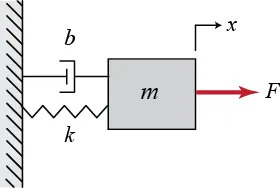
\includegraphics[width=0.35\textwidth]{Images/nonlinear/introduction/mass_spring_damper.jpg}
    \caption{Spring–mass–damper system with external force $F(t)$.}
    \label{fig:spring}
\end{figure}

Consider a mass $m$ attached to a spring (constant $k$) and damper (coefficient $b$), subject to an external force $F(t)$ as shown in the figure \ref{fig:spring}.  
The equation of motion is:
\begin{equation}
    m\ddot{x}(t) + b\dot{x}(t) + kx(t) = F(t).
\end{equation}

Defining the state vector as $x_1 = x(t)$ and $x_2 = \dot{x}(t)$, the system becomes:
\begin{align}
    \dot{x}_1 &= x_2, \\
    \dot{x}_2 &= -\tfrac{k}{m}x_1 - \tfrac{b}{m}x_2 + \tfrac{1}{m}F(t).
\end{align}

In matrix form:
\begin{equation}
\dot{x}(t) =
\begin{bmatrix}
0 & 1 \\
-\tfrac{k}{m} & -\tfrac{b}{m}
\end{bmatrix} x(t) +
\begin{bmatrix}
0 \\ \tfrac{1}{m}
\end{bmatrix} F(t),
\qquad
y(t) =
\begin{bmatrix}
1 & 0
\end{bmatrix} x(t).
\end{equation}
\end{example}

\section{Nonlinear Systems}\index{Nonlinear Systems}
\begin{definition}[Nonlinear System]
A general nonlinear system in state-space form is written as:
\begin{align}
    \dot{x} &= f\big(x,u,t\big), \\
    y &= g\big(x,u,t\big)
\end{align}
where $f(\cdot)$ and $g(\cdot)$ may depend explicitly on time $t$ in addition to the states $x$ and inputs $u$.
\end{definition}

\begin{example}[Spring–Mass–Damper with Nonlinear Spring]
Consider again the spring mass damper system as shown in figure \ref{fig:spring}, but now the spring has a nonlinear restoring force:
\begin{equation}
    F_{\text{spring}}(x) = k_1 x + k_3 x^3,
\end{equation}
so that the equation of motion becomes:
\begin{equation}
    m\ddot{x}(t) + b\dot{x}(t) + k_1 x(t) + k_3 x^3(t) = F(t).
\end{equation}

Defining $x_1 = x(t)$ and $x_2 = \dot{x}(t)$, the state equations are:
\begin{align}
    \dot{x}_1(t) &= x_2(t), \\
    \dot{x}_2(t) &= -\tfrac{b}{m}x_2(t) - \tfrac{k_1}{m}x_1(t) - \tfrac{k_3}{m}x_1^3(t) + \tfrac{1}{m}F(t).
\end{align}

Compactly,
\begin{equation}
\dot{x}(t) =
\begin{bmatrix}
x_2(t) \\
-\tfrac{b}{m}x_2(t) - \tfrac{k_1}{m}x_1(t) - \tfrac{k_3}{m}x_1^3(t) + \tfrac{1}{m}F(t)
\end{bmatrix},
\qquad
y(t) = x_1(t).
\end{equation}
\end{example}

\subsection{Special Cases}\index{Nonlinear Systems!Special Cases}
\begin{itemize}
    \item \textbf{Unforced System ($u(t)=0$):}  
    When $F(t)=0$, the dynamics reduce to:
    \begin{equation}
        \dot{x}_1 = x_2, \qquad 
        \dot{x}_2 = -\tfrac{b}{m}x_2 - \tfrac{k_1}{m}x_1 - \tfrac{k_3}{m}x_1^3.
    \end{equation}

    \item \textbf{Autonomous System ($\dot{x}=f(x)$):}  
    If the system has no input and no explicit time dependence,
    \begin{equation}
        \dot{x}(t) = f\big(x(t)\big).
    \end{equation}
    For this example,
    \begin{equation}
        \dot{x} =
        \begin{bmatrix}
        x_2 \\
        -\tfrac{b}{m}x_2 - \tfrac{k_1}{m}x_1 - \tfrac{k_3}{m}x_1^3
        \end{bmatrix}.
    \end{equation}
\end{itemize}

\section{Equilibrium Points}\index{Equilibrium Points}

\begin{definition}[Equilibrium Point]
An equilibrium point of a dynamical system
\begin{equation}
    \dot{x} = f(x,u,t),
\end{equation}
is a point $x_e$ (with corresponding input $u_e$) such that the state does not change in time:
\begin{equation}
    f(x_e,u_e,t) = 0, \qquad \forall t.
\end{equation}
In other words, if the system starts at $(x_e,u_e)$, it remains there for all time when there is no disturbance.
\end{definition}

\begin{example}[Spring–Mass–Damper with Nonlinear Spring]
For the nonlinear spring–mass–damper system
\begin{equation}
    \dot{x}_1 = x_2, \qquad 
    \dot{x}_2 = -\tfrac{b}{m}x_2 - \tfrac{k_1}{m}x_1 - \tfrac{k_3}{m}x_1^3 + \tfrac{1}{m}F(t),
\end{equation}
the equilibrium points are obtained by solving
\begin{align}
    0 &= x_2, \\
    0 &= -\tfrac{b}{m}x_2 - \tfrac{k_1}{m}x_1 - \tfrac{k_3}{m}x_1^3 + \tfrac{1}{m}F.
\end{align}

Thus, the equilibria satisfy
\begin{equation}
    -k_1 x_1 - k_3 x_1^3 + F = 0, \qquad x_2 = 0.
\end{equation}

\end{example}

\section{First-order Autonomous Nonlinear Systems}\index{First-order Autonomous Nonlinear Systems}

We consider systems of the form
\begin{equation}
    \dot{x} = f(x).
\end{equation}

\subsection{Linear Case}\index{First-order Autonomous Nonlinear Systems!Linear Case}
For a linear system
\begin{equation}
    \dot{x} = a x,
\end{equation}
the solution is
\begin{equation}
    x(t) = e^{at} x(0).
\end{equation}

\begin{itemize}
    \item If $a < 0$, the solution decays to zero (stable equilibrium).
    \item If $a > 0$, the solution diverges from zero (unstable equilibrium).
\end{itemize}

\subsection{General Nonlinear Case}\index{First-order Autonomous Nonlinear Systems!General Nonlinear Case}
For a general nonlinear function $f(x)$, an explicit analytical solution is often not possible.  
Instead, we examine the qualitative behavior by plotting $\dot{x} = f(x)$ as a function of $x$.  

\begin{example}[Nonlinear Example]
Consider
\begin{equation}
    \dot{x} = \cos x.
\end{equation}
Equilibrium points are given by $\cos x = 0$, i.e.
\[
x = \tfrac{\pi}{2} + n\pi, \quad n \in \mathbb{Z}.
\]
\end{example}

\begin{center}
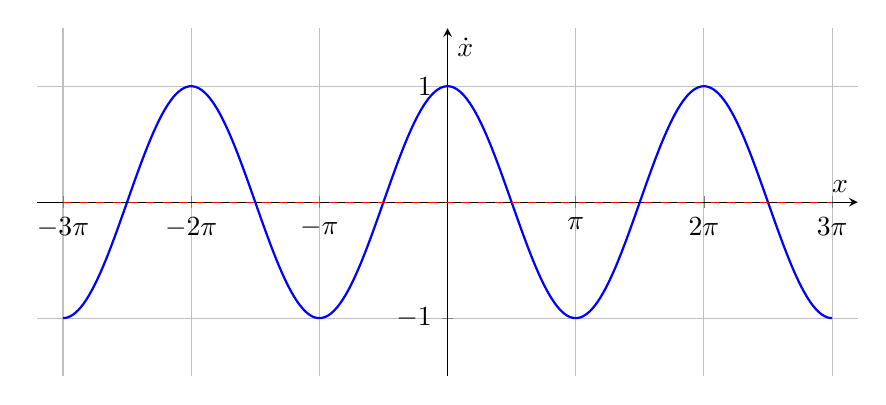
\begin{tikzpicture}[scale=1.0]
\begin{axis}[
    axis lines=middle,
    xlabel={$x$},
    ylabel={$\dot{x}$},
    domain=-3*pi:3*pi,
    samples=300,
    width=12cm,
    height=6cm,
    grid=both,
    xmin=-3.2*pi, xmax=3.2*pi,
    ymin=-1.5, ymax=1.5,
    xtick={-9.425,-6.283,-3.142,0,3.142,6.283,9.425},
    xticklabels={$-3\pi$,$-2\pi$,$-\pi$,0,$\pi$,$2\pi$,$3\pi$},
    ytick={-1,0,1}
]
\addplot[blue, thick] {cos(deg(x))};
\draw[dashed, red] (-3*pi,0) -- (3*pi,0); % equilibrium reference line
\end{axis}
\end{tikzpicture}
\end{center}

From the plot we observe:
\begin{itemize}
    \item Where $\dot{x} > 0$, the trajectories increase.
    \item Where $\dot{x} < 0$, the trajectories decrease.
    \item Equilibria occur at zeros of $f(x)$, and their stability depends on the slope $f'(x)$.
\end{itemize}

\section{Second-Order Systems: Phase-Plane Analysis}\index{Second-Order Systems: Phase-Plane Analysis}

\begin{definition}[Phase-Plane Analysis]
Phase-plane analysis is a qualitative method for studying second-order dynamical systems of the form
\begin{align}
    \dot{x}_1 &= f_1(x_1, x_2), \\
    \dot{x}_2 &= f_2(x_1, x_2).
\end{align}
The system’s behavior is analyzed in the $(x_1,x_2)$ plane, called the \emph{phase plane}, where each point corresponds to a state of the system.  
The direction field (or vector field) indicates the slope of trajectories at each point, and integral curves show the system trajectories.
\end{definition}

\subsection{Methodology}\index{Second-Order Systems: Phase-Plane Analysis!Methodology}
To perform phase-plane analysis:
\begin{enumerate}
    \item Write the system as two first-order equations in variables $(x_1, x_2)$.
    \item Identify equilibrium points by solving $\dot{x}_1=0, \; \dot{x}_2=0$.
    \item At each point $(x_1,x_2)$, compute $(\dot{x}_1,\dot{x}_2)$ and draw the vector field.
    \item Sketch trajectories (integral curves) that follow these vectors.
\end{enumerate}

\begin{example}[Nonlinear System]
\begin{figure}[h!]
    \centering
    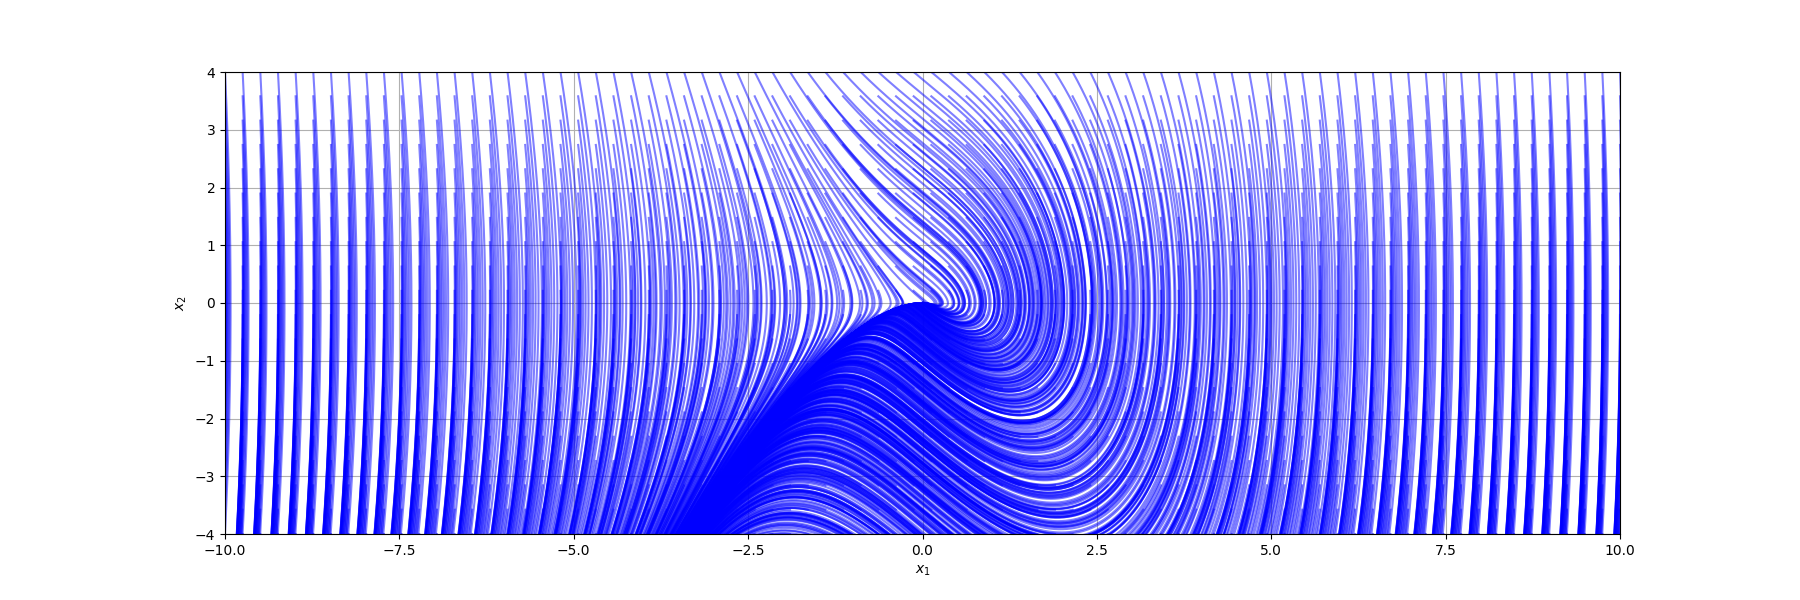
\includegraphics[width=\linewidth]{Images/nonlinear/introduction/phase.png}
    \caption{Phase portrait}
    \label{fig:phase}
\end{figure}
Consider the system
\begin{align}
    \dot{x}_1 &= x_2, \\
    \dot{x}_2 &= -x_1^2 - x_2.
\end{align}
\\
\textbf{Step 1: Equilibrium Points.}  
\\Solve
\[
x_2 = 0, \qquad -x_1^2 - x_2 = 0.
\]
This gives the only equilibrium at $(x_1, x_2) = (0,0)$.
\\\\
\textbf{Step 2: Vector Field.}  
\\The vector field in the $(x_1,x_2)$ plane is obtained (as shown in figure \ref{fig:phase}) by evaluating
\[
\dot{x}_1 = x_2, \qquad \dot{x}_2 = -x_1^2 - x_2.
\]


\textbf{Observation.}  
- The equilibrium at $(0,0)$ is asymptotically stable, since $x_2$ introduces damping and $-x_1^2$ is always nonpositive.  
- Trajectories spiral or curve toward the origin but with nonlinear effects due to the $-x_1^2$ term.
\end{example}

\section{Phase-Plane Analysis of LTI Systems}\index{Phase-Plane Analysis of LTI Systems}

We now specialize phase-plane analysis to \emph{linear time-invariant (LTI)} systems of the form
\begin{equation}
    \dot{x}(t) = A x(t), \qquad A \in \mathbb{R}^{2\times 2}.
\end{equation}
The solution is
\begin{equation}
    x(t) = e^{At} x(0).
\end{equation}
The qualitative behavior depends only on the eigenvalues of $A$.  

\subsection{Case 1: Diagonalizable Systems with Real Eigenvalues}\index{Phase-Plane Analysis of LTI Systems!Case 1}

Suppose $A$ has two distinct real eigenvalues $\lambda_1, \lambda_2$ with corresponding linearly independent eigenvectors $v_1, v_2$.  
Then, $A$ is diagonalizable:
\[
A = T D T^{-1}, \qquad D = \text{diag}(\lambda_1,\lambda_2),
\]
so that in the transformed coordinates $z = T^{-1}x$,
\[
\dot{z} = Dz =
\begin{bmatrix}
\lambda_1 & 0 \\
0 & \lambda_2
\end{bmatrix} z.
\]

The solutions are
\[
z_1(t) = z_1(0)e^{\lambda_1 t}, \qquad z_2(t) = z_2(0)e^{\lambda_2 t}.
\]

\paragraph{Qualitative Behavior.}
\begin{itemize}
    \item If $\lambda_1, \lambda_2 < 0$: trajectories decay to the origin (stable node).
    \item If $\lambda_1, \lambda_2 > 0$: trajectories diverge (unstable node).
    \item If $\lambda_1 \lambda_2 < 0$: trajectories approach along the stable direction and diverge along the unstable one (saddle point).
\end{itemize}

The eigenvectors define the principal axes of trajectories in the phase plane.

\subsection{Case 2: Non-Diagonalizable Systems (Defective Matrix)}\index{Phase-Plane Analysis of LTI Systems!Case 2}

If $A$ has a repeated eigenvalue $\lambda$ but only one independent eigenvector, then it is not diagonalizable.  
Instead, we form the Jordan form:
\[
A = P J P^{-1}, \qquad J =
\begin{bmatrix}
\lambda & 1 \\
0 & \lambda
\end{bmatrix}.
\]

The solution in Jordan coordinates is
\[
z(t) =
\begin{bmatrix}
e^{\lambda t} & t e^{\lambda t} \\
0 & e^{\lambda t}
\end{bmatrix} z(0).
\]

\paragraph{Qualitative Behavior.}
\begin{itemize}
    \item If $\lambda < 0$: trajectories decay to the origin but not along straight lines; they are distorted due to the $t e^{\lambda t}$ term.
    \item If $\lambda > 0$: trajectories diverge with polynomially growing components.
    \item If $\lambda = 0$: trajectories grow linearly with $t$ (marginal stability).
\end{itemize}

In the phase plane, trajectories are tangent to the single eigenvector direction but curve due to the generalized eigenvector contribution.

\subsection{Case 3: Systems with Complex Eigenvalues}\index{Phase-Plane Analysis of LTI Systems!Case 3}

If $A$ has complex-conjugate eigenvalues $\lambda_{1,2} = \alpha \pm j\beta$ with $\beta \neq 0$, then $A$ can be transformed into
\[
M^{-1} A M =
\begin{bmatrix}
\alpha & -\beta \\
\beta & \alpha
\end{bmatrix}.
\]

The solution is
\[
z(t) = e^{\alpha t}
\begin{bmatrix}
\cos(\beta t) & -\sin(\beta t) \\
\sin(\beta t) & \cos(\beta t)
\end{bmatrix} z(0).
\]

\paragraph{Qualitative Behavior.}
\begin{itemize}
    \item If $\alpha < 0$: trajectories spiral into the origin (stable focus).
    \item If $\alpha > 0$: trajectories spiral outward (unstable focus).
    \item If $\alpha = 0$: trajectories form closed orbits (center, neutrally stable).
\end{itemize}

The frequency of oscillation is $\beta$, and $\alpha$ determines whether the spiral converges or diverges.

\begin{example}[Comparison of LTI Systems]
\begin{figure}[h!]
    \centering
    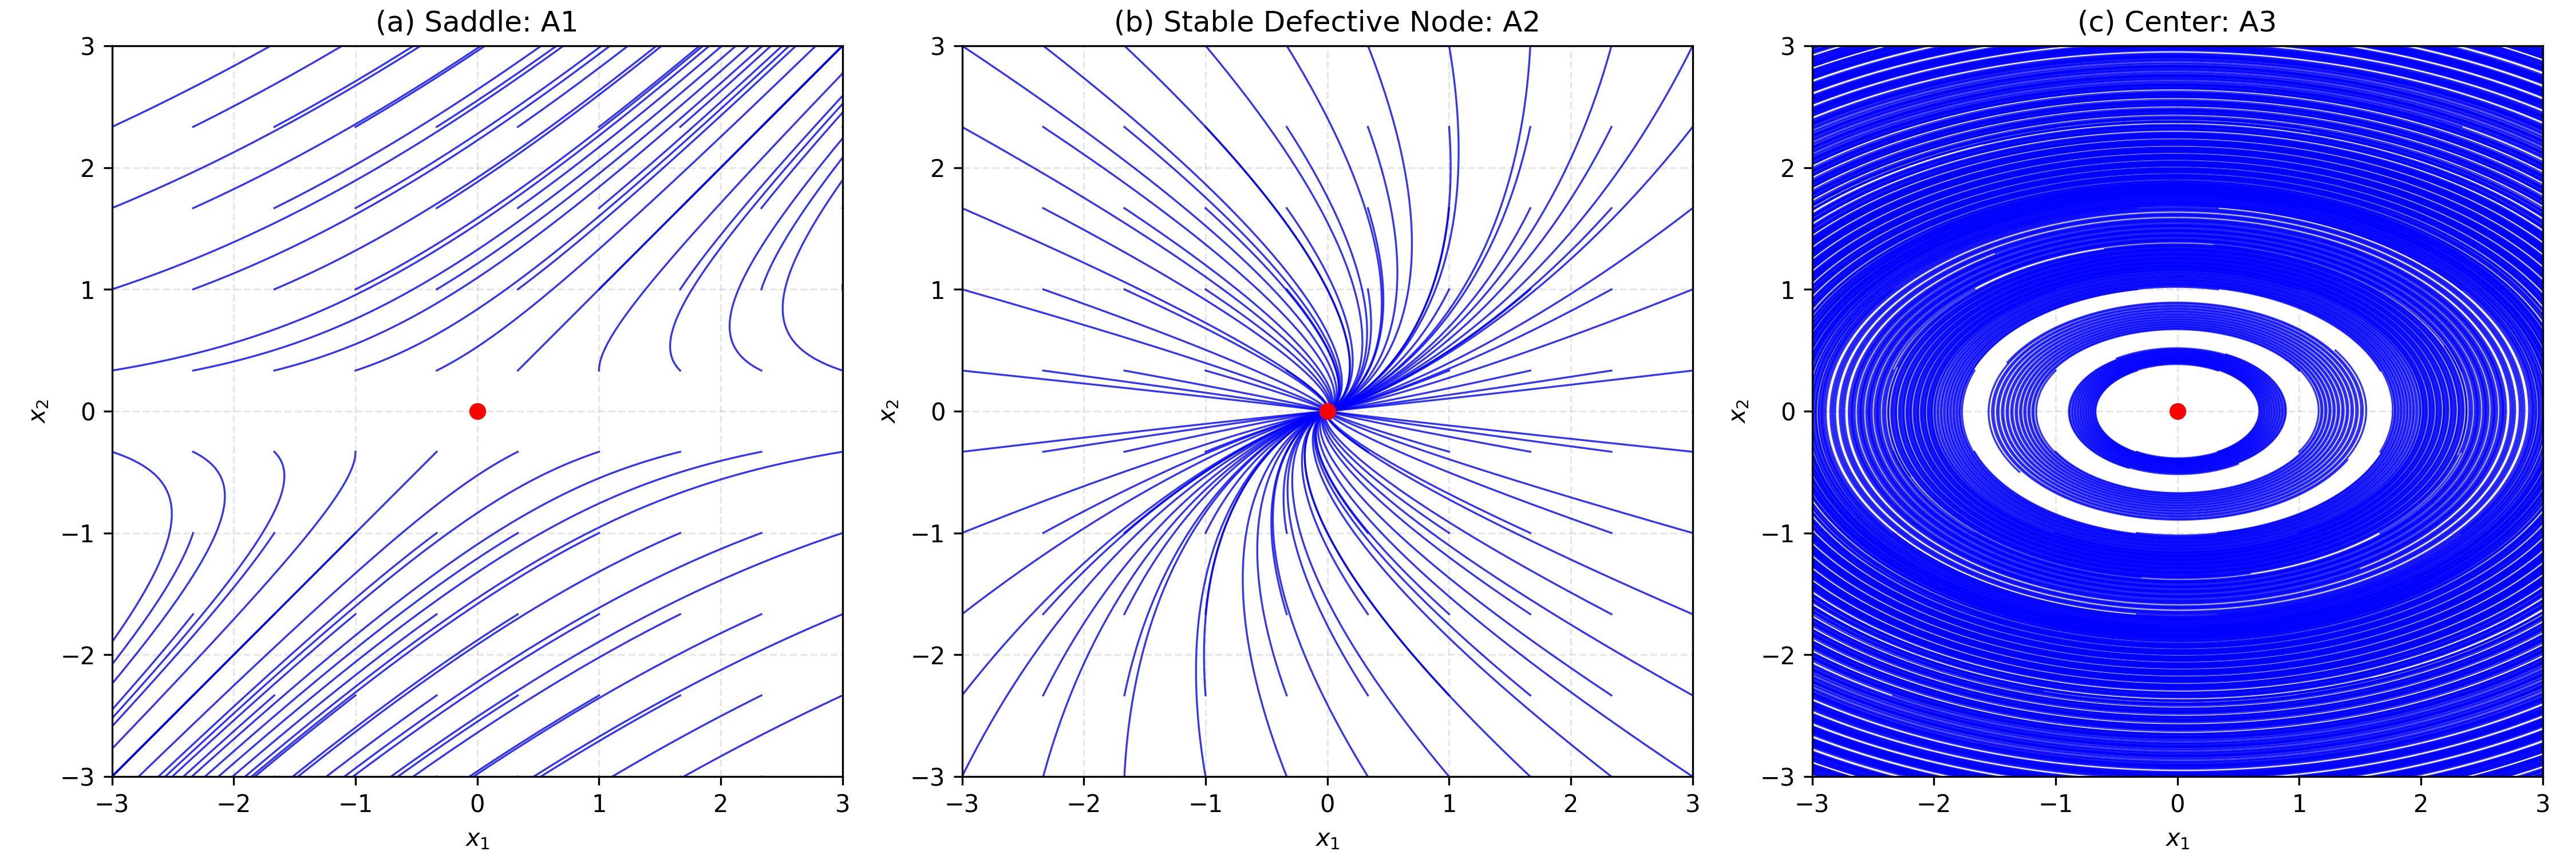
\includegraphics[width=\linewidth]{Images/nonlinear/introduction/phase_dense.png}
    \caption{Phase portraits of three different LTI systems: 
    (a) saddle point, 
    (b) stable defective node, 
    (c) center.}
    \label{fig:lti_phase}
\end{figure}

We compare the qualitative behavior of three linear time-invariant systems of the form
\[
\dot{x}(t) = A x(t), \qquad A \in \mathbb{R}^{2\times 2}.
\]

\textbf{Case 1: Saddle Point.}  
\[
A_1 = \begin{bmatrix} -1 & 3 \\ 0 & 2 \end{bmatrix}.
\]
Eigenvalues are $\lambda_1=-1$, $\lambda_2=2$ with opposite signs.  
Trajectories approach the origin along the stable direction and diverge along the unstable one, forming a saddle (Fig.~\ref{fig:lti_phase}a).

\textbf{Case 2: Stable Defective Node.}  
\[
A_2 = \begin{bmatrix} -2 & 1 \\ 0 & -2 \end{bmatrix}.
\]
This has a repeated eigenvalue $\lambda=-2$ with only one eigenvector.  
Trajectories converge to the origin but are distorted due to the Jordan block structure, curving toward the equilibrium (Fig.~\ref{fig:lti_phase}b).

\textbf{Case 3: Center.}  
\[
A_3 = \begin{bmatrix} 0 & -3 \\ 1 & 0 \end{bmatrix}.
\]
Eigenvalues are purely imaginary $\lambda = \pm j\sqrt{3}$.  
Trajectories form closed orbits, indicating a neutrally stable center (Fig.~\ref{fig:lti_phase}c).
\end{example}

\subsection{Conclusion}\index{Phase-Plane Analysis of LTI Systems!Conclusion}
\begin{table}[h!]
    \centering
    \begin{tabular}{|c|c|}\hline
         \textbf{Eigenvalues} & \textbf{Equilibrium type} \\\hline
         $\lambda_1,\lambda_2$ real, both $<0$ & Stable node \\\hline
         $\lambda_1,\lambda_2$ real, both $>0$ & Unstable node \\\hline
         $\lambda_1\lambda_2 < 0$ (real, opposite signs) & Saddle point \\\hline
         Complex with $\Re(\lambda)<0$ & Stable focus (spiral in) \\\hline
         Complex with $\Re(\lambda)>0$ & Unstable focus (spiral out) \\\hline
         Purely imaginary ($\Re(\lambda)=0$) & Center (neutrally stable) \\\hline
    \end{tabular}
    \caption{Summary of different equilibrium cases for $2\times2$ LTI systems.}
    \label{tab:lti_summary}
\end{table}

\section{Phase Plane Analysis of Nonlinear Systems}\index{Phase Plane Analysis of Nonlinear Systems}

Unlike linear systems, nonlinear systems often exhibit phenomena such as 
\emph{self-excited oscillations}. These oscillations do not require external forcing
and are called \textbf{limit cycles}. A limit cycle is a closed trajectory in the 
phase plane that is isolated, meaning nearby trajectories either spiral towards it 
(stable) or away from it (unstable). 

\subsection{Limit Cycles}\index{Phase Plane Analysis of Nonlinear Systems!Limit Cycles}

One of the most famous examples of a system with a limit cycle is the 
\textbf{Van der Pol oscillator}.

\begin{definition}[Van der Pol Oscillator]
    The Van der Pol oscillator is governed by the second-order nonlinear differential equation
    \begin{equation}
        \ddot{x} - \mu(1-x^2)\dot{x} + x = 0, \qquad \mu \geq 0
    \end{equation}
    where $\mu$ is a scalar parameter controlling nonlinearity and damping.
\end{definition}

\subsubsection*{State-Space Form}
Let $x_1 = x$ and $x_2 = \dot{x}$, then
\begin{align}
    \dot{x}_1 &= x_2 \\
    \dot{x}_2 &= \mu(1 - x_1^2)x_2 - x_1
\end{align}
This defines the nonlinear vector field:
\[
\dot{\mathbf{x}} =
\begin{bmatrix}
x_2 \\
\mu(1-x_1^2)x_2 - x_1
\end{bmatrix}.
\]

\subsubsection*{Equilibrium and Dynamics}
\begin{remark}
    For $\mu = 0$, the system reduces to the linear oscillator
    \begin{equation}
        \dot{x}_1 = x_2, \qquad \dot{x}_2 = -x_1,
    \end{equation}
    which has the origin $(0,0)$ as a center with closed trajectories (neutrally stable).
\end{remark}

\begin{remark}
    For $\mu > 0$, the nonlinear term $\mu(1-x_1^2)x_2$ introduces:
    \begin{itemize}
        \item Negative damping near the origin, pushing trajectories outward.
        \item Positive damping for large $|x_1|$, pulling trajectories inward.
    \end{itemize}
    This balance creates a \textbf{stable limit cycle}, i.e. all trajectories converge to a periodic orbit.
\end{remark}

\begin{example}[Vector Field of Van der Pol Oscillator: Stable vs. Unstable]
    The Van der Pol oscillator in state-space form is
    \begin{align}
        \dot{x}_1 &= x_2 \\
        \dot{x}_2 &= \pm \mu (1-x_1^2)x_2 - x_1,
    \end{align}
    where the choice of sign determines the nature of the dynamics:
    \begin{itemize}
        \item With $+\mu$, the system exhibits a \textbf{stable limit cycle}, attracting trajectories.  
        \item With $-\mu$, the system exhibits an \textbf{unstable limit cycle}, repelling trajectories.  
    \end{itemize}

    The corresponding vector fields for $\mu=1$ are shown below.

    \begin{figure}[h!]
        \centering
        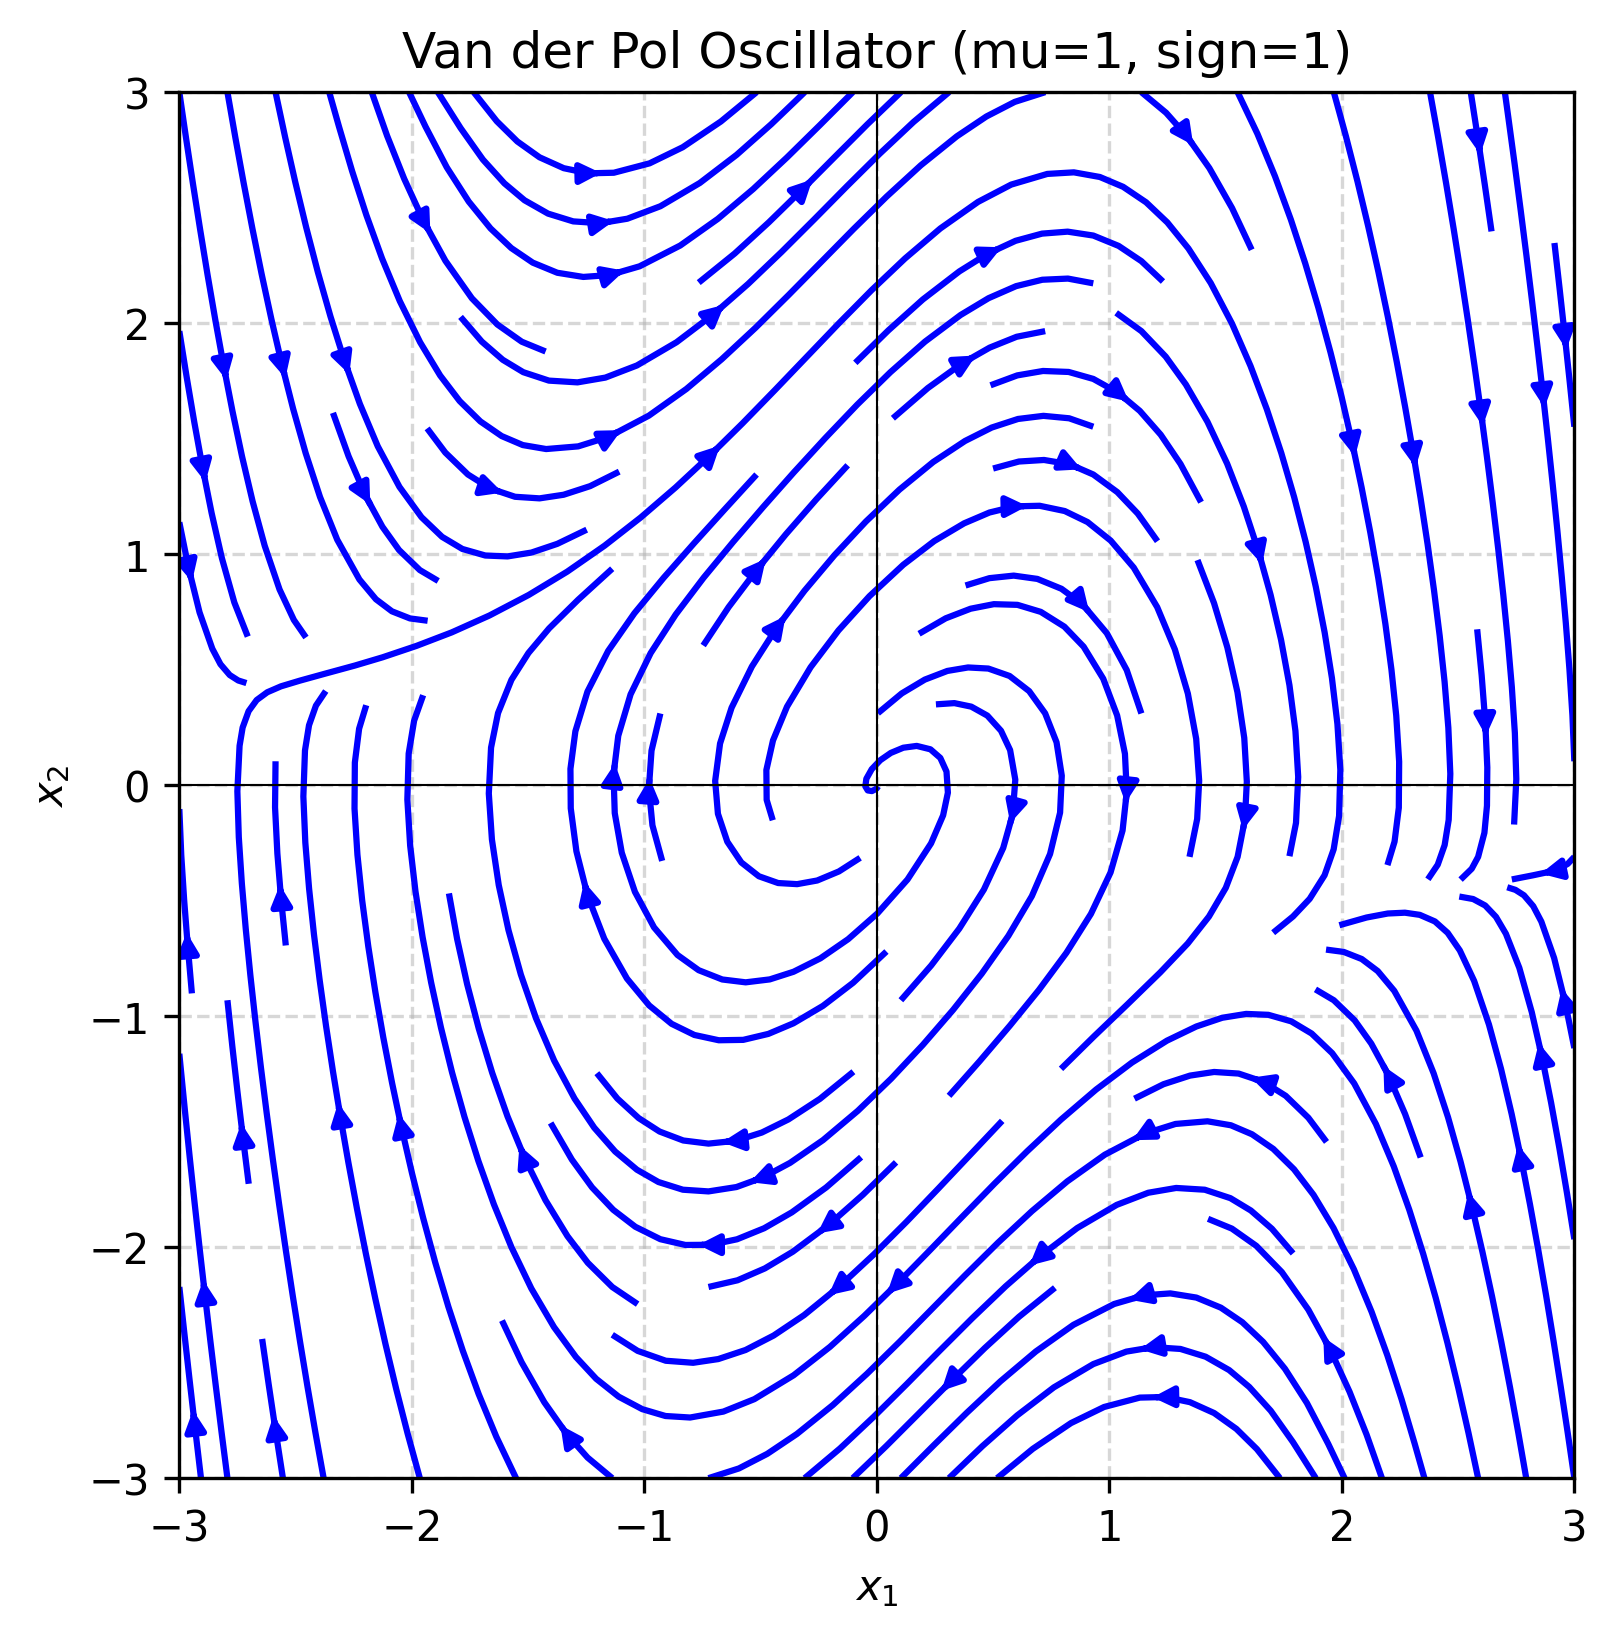
\includegraphics[width=0.4\textwidth]{Images/nonlinear/introduction/vdp_stable.png}
        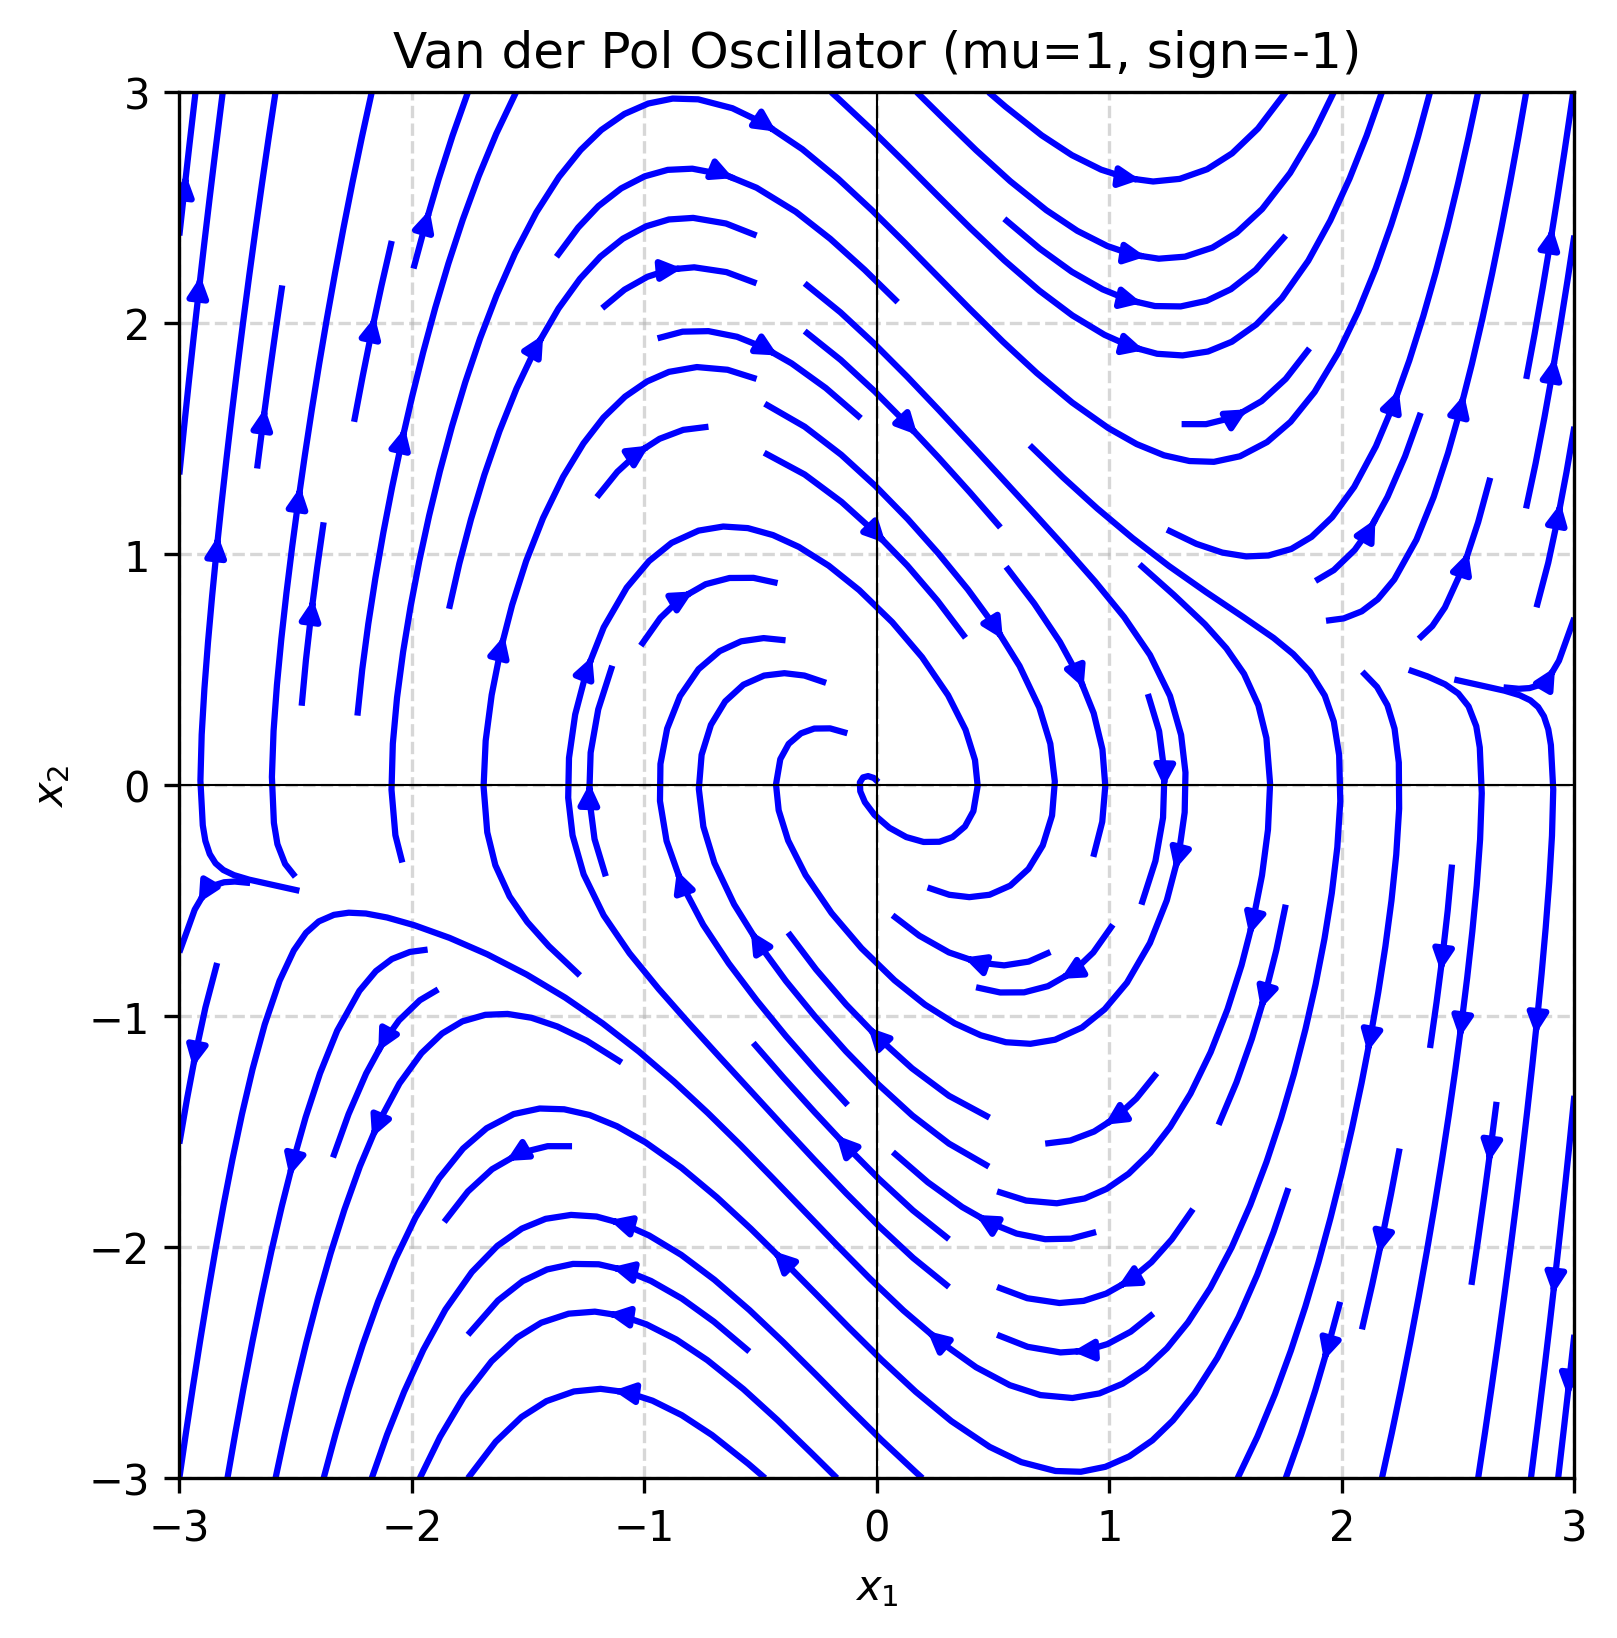
\includegraphics[width=0.4\textwidth]{Images/nonlinear/introduction/vdp_unstable.png}
        \caption{Phase portraits of the Van der Pol oscillator for $\mu=1$: stable limit cycle (left) and unstable limit cycle (right).}
    \end{figure}
\end{example}


\begin{remark}
A \textbf{stable limit cycle} attracts nearby trajectories, an \textbf{unstable limit cycle} repels them, and a \textbf{semistable limit cycle} attracts trajectories on one side while repelling on the other. 
\end{remark}

